\documentclass[11pt]{article}

\usepackage[margin=1in]{geometry}
\usepackage{amsmath,amssymb}
\usepackage{booktabs}
\usepackage{graphicx}
\usepackage{float}
\usepackage{hyperref}
\usepackage{setspace}
\usepackage[european]{circuitikz}

\hypersetup{
  colorlinks=true,
  linkcolor=blue,
  urlcolor=blue,
  citecolor=blue
}

\begin{document}
\onehalfspacing
\pagenumbering{gobble}

\begin{titlepage}
    \centering
    \vspace*{0.24\textheight}
    {\LARGE Theory Behind Simulations\par}
    \vspace{1.5cm}
    {\Large Single VO2 Neuristor under Voltage and Current Sources\par}
    \vfill
    {\large by Gabriel Berezovsky\par}
    \vspace*{0.1\textheight}
\end{titlepage}

\clearpage
\pagenumbering{roman}
\tableofcontents
\clearpage
\pagenumbering{arabic}

\section{Introduction}

\begin{figure}[htbp]
\centering
\begin{circuitikz}
% Vin -> Rload -> node V (left to right)
\draw (0,0) node[ocirc]{} node[left]{\(V_{in}\)}
      to[R, l=\(R_{\mathrm{load}}\)] (3,0)
      node[circ]{} node[above left]{\(V\)} coordinate (Vnode);

% RC block: both source-side and ground-side tied at side midpoints
\coordinate (LeftTop) at (3.0,0.9);
\coordinate (LeftBot) at (3.0,-0.9);
\coordinate (RightTop) at (5.4,0.9);
\coordinate (RightMid) at (5.4,0.0);
\coordinate (RightBot) at (5.4,-0.9);

% Vertical side rails (midpoint connection at V on the left)
\draw (LeftTop) -- (Vnode) -- (LeftBot);
\draw (RightTop) -- (RightMid) -- (RightBot);

% Top and bottom horizontal branches
\draw (LeftTop) to[C, l=\(C\)] (RightTop);
\draw (LeftBot) to[R, l=\(R\)] (RightBot);

% Ground lead from right midpoint: right first, then down
\draw (RightMid) -- (6.2,0) -- (6.2,-2.2) node[ground]{};
\end{circuitikz}
\caption{Single-neuristor equivalent circuit used in the voltage-driven model.}
\label{fig:intro_single_neuristor_circuit}
\end{figure}

\subsection{Current Dynamics Equation}
\subsubsection*{Equation(s)}
Source equation (Zhang \emph{et al.}, 2024):
\begin{equation}
C\frac{dV_i}{dt}=\frac{V^{in}_i}{R^{load}_i}-V_i\left(\frac{1}{R_i}+\frac{1}{R^{load}_i}\right).
\label{eq:intro_current_original}
\end{equation}

Single-device form used in this project:
\begin{equation}
C\frac{dV}{dt}=\frac{V_{in}}{R_{series}}-V\left(\frac{1}{R_{vo2}}+\frac{1}{R_{series}}\right),
\quad R_{vo2}=R(T,\mathcal{H}),
\label{eq:intro_current_single}
\end{equation}
\begin{equation}
\frac{dV}{dt}=\frac{V_{in}-V}{R_{series}C}-\frac{V}{R_{vo2}C}.
\label{eq:intro_current_single_rearranged}
\end{equation}

\subsubsection*{Variables and Units}
\begin{center}
\begin{tabular}{lll}
\toprule
Symbol & Meaning & Units \\
\midrule
\(V_i, V\) & node/device voltage across VO\textsubscript{2} and capacitor & V \\
\(V^{in}_i, V_{in}\) & applied source voltage & V \\
\(R_i, R_{vo2}\) & VO\textsubscript{2} resistance state & \(\Omega\) \\
\(R^{load}_i, R_{series}\) & series/load resistance & \(\Omega\) \\
\(C\) & parasitic/effective node capacitance & F \\
\(t\) & time & s \\
\(\mathcal{H}\) & hysteresis internal state (branch/reversal memory) & -- \\
\bottomrule
\end{tabular}
\end{center}

\subsubsection*{Physical Interpretation}
\begin{itemize}
    \item \(C\,dV/dt\): capacitive storage term (how fast node voltage can change).
    \item Source-branch current is \(I_{src}=(V_{in}-V)/R_{series}\), which can be decomposed as \(V_{in}/R_{series}-V/R_{series}\).
    \item \(V/R_{series}\): the part of the source-branch term that opposes charging as node voltage rises.
    \item \(V/R_{vo2}\): current through the VO\textsubscript{2} device; this term is strongly nonlinear because \(R_{vo2}\) depends on temperature and hysteresis state.
\end{itemize}
The competition between \(I_{src}=(V_{in}-V)/R_{series}\) and VO\textsubscript{2} discharge determines oscillatory charging--switching dynamics.

\subsection{Thermal Dynamics Equation}
\subsubsection*{Equation(s)}
Source equation (Zhang \emph{et al.}, 2024):
\begin{equation}
C_{th}\frac{dT_i}{dt}=\frac{V_i^2}{R_i}-S_e(T_i-T_0)+S_c\nabla^2T_i+\sigma\eta_i(t).
\label{eq:intro_thermal_original}
\end{equation}

Single-device reduction (\(\nabla^2T=0\)):
\begin{equation}
C_{th}\frac{dT}{dt}=\frac{V^2}{R_{vo2}}-S_e(T-T_0)+\sigma\eta(t).
\label{eq:intro_thermal_single}
\end{equation}

\subsubsection*{Variables and Units}
\begin{center}
\begin{tabular}{lll}
\toprule
Symbol & Meaning & Units \\
\midrule
\(T_i, T\) & device temperature & K \\
\(t\) & time & s \\
\(C_{th}\) & thermal capacitance & J/K \\
\(V_i, V\) & device voltage & V \\
\(R_i, R_{vo2}\) & VO\textsubscript{2} resistance & \(\Omega\) \\
\(S_e\) & thermal conductance to environment/substrate & W/K \\
\(S_c\) & nearest-neighbor thermal coupling conductance & W/K \\
\(T_0\) & ambient/base temperature & K \\
\(\nabla^2T\) & discrete thermal Laplacian (neighbor exchange term) & K \\
\(\eta_i(t)\) & Gaussian white-noise process (paper notation) & s\(^{-1/2}\) \\
\(\sigma\) & noise strength multiplier (paper notation) & J\,s\(^{-1/2}\) \\
\bottomrule
\end{tabular}
\end{center}

\subsubsection*{Physical Interpretation}
\begin{itemize}
    \item \(\frac{V^2}{R_{vo2}}\): Joule-heating input that increases \(T\).
    \item \(S_e(T-T_0)\): heat leakage to ambient that decreases \(T\) when \(T>T_0\).
    \item \(S_c\nabla^2T\): diffusive thermal exchange with neighbors; positive when neighbors are hotter.
    \item \(\sigma\eta_i(t)\): stochastic thermal fluctuations (paper noise term).
\end{itemize}
The thermal equation therefore balances Joule heating, environmental cooling, inter-device heat diffusion, and noise.

\subsection{Resistance / Hysteresis Model}
\begin{figure}[htbp]
\centering
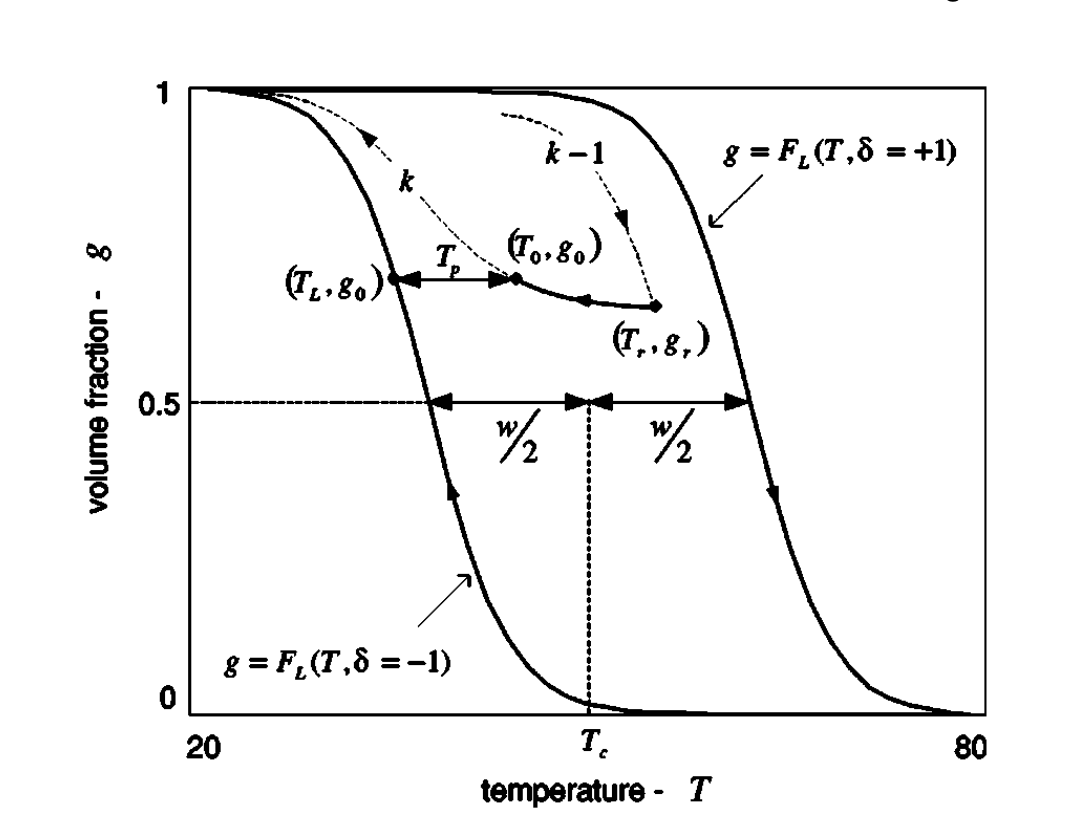
\includegraphics[width=0.78\textwidth]{figures/hysteresis.png}
\caption{Reference hysteresis geometry showing major branches, reversal points, and proximity temperature shift in the volume-fraction model.}
\label{fig:resistance_hysteresis_geometry}
\end{figure}

\subsubsection*{Equation(s)}
Starting point from de Almeida \emph{et al.} (2002):
\begin{equation}
R_s(T)=R_0\exp\!\left(\frac{E_a}{k_B T}\right).
\label{eq:intro_res_rs}
\end{equation}
\begin{equation}
R(T)\approx g(T)R_s(T)+(1-g(T))R_m
\;\;\Rightarrow\;\;
R(T)\approx g(T)R_s(T)+R_m.
\label{eq:intro_res_mix}
\end{equation}

Major-loop semiconducting fraction:
\begin{equation}
g_{\mathrm{major}}(T,\delta)=\frac{1}{2}+\frac{1}{2}\tanh\!\left[\beta\left(\delta\frac{w}{2}+T_c-T\right)\right],
\quad
\delta=\begin{cases}
+1,& dT/dt>0,\\
-1,& dT/dt<0.
\end{cases}
\label{eq:intro_res_major}
\end{equation}

Minor-loop memory terms:
\begin{equation}
T_{pr}=\delta\frac{w}{2}+T_c-\frac{1}{\beta}\operatorname{arctanh}(2g_r-1)-T_r,
\label{eq:intro_res_tpr}
\end{equation}
\begin{equation}
x=\frac{T-T_r}{T_{pr}},
\qquad
P(x)=\frac{1}{2}\left(1-\sin(\gamma x)\right)\left(1+\tanh(\pi^2-2\pi x)\right),
\qquad
T_p=T_{pr}P(x),
\label{eq:intro_res_proximity}
\end{equation}
\begin{equation}
g(T,\mathcal{H})=\frac{1}{2}+\frac{1}{2}\tanh\!\left[\beta\left(\delta\frac{w}{2}+T_c-(T+T_p)\right)\right].
\label{eq:intro_res_minor}
\end{equation}

Final resistance law used in this project:
\begin{equation}
R_{vo2}(T,\mathcal{H})=R_0\exp\!\left(\frac{E_a/k_B}{T}\right)g(T,\mathcal{H})+R_m.
\label{eq:intro_res_final}
\end{equation}

\subsubsection*{Variables and Units}
\begin{center}
\begin{tabular}{lll}
\toprule
Symbol & Meaning & Units \\
\midrule
\(R_{vo2},R(T)\) & VO\textsubscript{2} device resistance & \(\Omega\) \\
\(R_s(T)\) & semiconducting-branch resistance (Arrhenius) & \(\Omega\) \\
\(R_m\) & metallic-state resistance floor & \(\Omega\) \\
\(R_0\) & Arrhenius prefactor & \(\Omega\) \\
\(E_a/k_B\) & activation-energy-over-Boltzmann term & K \\
\(T\) & device temperature (our model: Kelvin) & K \\
\(g(T,\mathcal{H})\) & semiconducting volume fraction with hysteresis memory & -- \\
\(w\) & hysteresis width parameter & K \\
\(T_c\) & hysteresis center temperature & K \\
\(\beta\) & branch steepness & K\(^{-1}\) \\
\(\delta\) & branch sign (\(+1\) heating, \(-1\) cooling) & -- \\
\(T_r,g_r\) & last reversal state (temperature, fraction) & K, -- \\
\(T_{pr}\) & reversal-derived proximity temperature scale & K \\
\(\gamma\) & proximity-function shape parameter & -- \\
\(P(x)\) & proximity function controlling minor-loop approach & -- \\
\(T_p\) & instantaneous proximity temperature shift & K \\
\(\mathcal{H}\) & full hysteresis state \((\delta,T_r,g_r,T_{pr},\ldots)\) & -- \\
\(\tilde R,\tilde g\) & measured resistance and inferred fraction for fitting & \(\Omega\), -- \\
\bottomrule
\end{tabular}
\end{center}

\subsubsection*{Physical Interpretation}
\begin{itemize}
    \item Eq.~\eqref{eq:intro_res_rs}: \(R_s(T)\) decreases exponentially with temperature in the insulating/semiconducting regime.
    \item Eq.~\eqref{eq:intro_res_mix}: total resistance combines semiconducting contribution \(gR_s\) with a metallic floor \(R_m\).
    \item Eq.~\eqref{eq:intro_res_major}: two major branches are selected by \(\delta\), creating the loop width \(w\).
    \item Eqs.~\eqref{eq:intro_res_tpr}--\eqref{eq:intro_res_proximity}: reversal variables \((T_r,g_r,T_{pr})\) and \(P(x)\) encode memory and generate minor loops.
    \item Eq.~\eqref{eq:intro_res_final}: this is the resistance passed to the electrical/thermal ODEs at every timestep.
\end{itemize}

\subsubsection*{Assumptions}
\begin{itemize}
    \item \(R_s\gg R_m\) in the transition regime justifies the additive form in Eq.~\eqref{eq:intro_res_mix}.
    \item Major-loop branches are represented by a symmetric \(\tanh\) form around \(T_c\).
    \item Hysteresis state updates only at reversal events (\(dT/dt\) sign change).
\end{itemize}

\section{Derivation of the Current-Source Model}

\subsection{Starting Point: Original Voltage-Driven Equations}
\subsubsection*{Equation(s)}
\begin{equation}
C\frac{dV}{dt}=\frac{V_{in}}{R_{series}}-V\left(\frac{1}{R_{vo2}}+\frac{1}{R_{series}}\right),
\qquad
R_{vo2}=R(T,\mathcal{H}).
\label{eq:sec2_start_electrical}
\end{equation}
\begin{equation}
C_{th}\frac{dT}{dt}=\frac{V^2}{R_{vo2}}-S_e(T-T_0)+\sigma\eta(t).
\label{eq:sec2_start_thermal}
\end{equation}

\subsection{Assumptions and Circuit Interpretation}
\subsubsection*{Assumptions}
\begin{itemize}
    \item The voltage source is removed and replaced by a current source in a separate experiment.
    \item The source enforces an ideal programmed current waveform \(I_{in}(t)\).
    \item An external resistor \(R_{series}\) may be present in the injection path in the physical setup.
    \item Under ideal current drive, adding/removing this external \(R_{series}\) does not change node-current balance, so both circuits are dynamically equivalent.
    \item The VO\textsubscript{2} branch representation is unchanged: \(R_{vo2}(T,\mathcal{H})\) in parallel with \(C\), referenced to ground.
    \item Thermal dynamics keeps the same Joule-heating/cooling structure as in Section 1.2.
\end{itemize}

\begin{figure}[htbp]
\centering
\begin{minipage}[c]{0.44\textwidth}
\centering
\begin{circuitikz}[scale=0.82]
% Physical setup: ideal current source + external series resistor
\coordinate (Sbot) at (0,-2.0);
\node[draw,circle,minimum size=0.75cm,inner sep=0pt] (IsrcA) at (0,-0.8) {};
\draw (Sbot) -- (IsrcA.south);
\draw (IsrcA.north) -- (0,0)
      to[R, l=\(R_{series}\)] (2.4,0)
      node[circ]{} node[above left]{\(V\)} coordinate (Va);
\draw[->] (0,-1.0) -- (0,-0.6);
\node[left] at (-0.15,-0.8) {\(I_{in}\)};

\coordinate (ALT) at (2.4,0.8);
\coordinate (ALB) at (2.4,-0.8);
\coordinate (ART) at (4.7,0.8);
\coordinate (ARM) at (4.7,0.0);
\coordinate (ARB) at (4.7,-0.8);
\draw (ALT) -- (Va) -- (ALB);
\draw (ART) -- (ARM) -- (ARB);
\draw (ALT) to[C, l=\(C\)] (ART);
\draw (ALB) to[R, l=\(R_{vo2}\)] (ARB);
\draw (ARM) -- (5.4,0) -- (5.4,-2.0) -- (Sbot);
\draw (2.9,-2.0) node[ground]{};
\end{circuitikz}

\vspace{1mm}
{\footnotesize Physical setup (with external \(R_{series}\))}
\end{minipage}
\hfill
\begin{minipage}[c]{0.08\textwidth}
\centering
\[
\Longrightarrow
\]
\end{minipage}
\hfill
\begin{minipage}[c]{0.44\textwidth}
\centering
\begin{circuitikz}[scale=0.82]
% Dynamical equivalent: same circuit with R_series replaced by a short
\coordinate (SbotB) at (0,-2.0);
\node[draw,circle,minimum size=0.75cm,inner sep=0pt] (IsrcB) at (0,-0.8) {};
\draw (SbotB) -- (IsrcB.south);
\draw (IsrcB.north) -- (0,0) -- (2.4,0)
      node[circ]{} node[above left]{\(V\)} coordinate (Vb);
\draw[->] (0,-1.0) -- (0,-0.6);
\node[left] at (-0.15,-0.8) {\(I_{in}\)};

\coordinate (BLT) at (2.4,0.8);
\coordinate (BLB) at (2.4,-0.8);
\coordinate (BRT) at (4.7,0.8);
\coordinate (BRM) at (4.7,0.0);
\coordinate (BRB) at (4.7,-0.8);
\draw (BLT) -- (Vb) -- (BLB);
\draw (BRT) -- (BRM) -- (BRB);
\draw (BLT) to[C, l=\(C\)] (BRT);
\draw (BLB) to[R, l=\(R_{vo2}\)] (BRB);
\draw (BRM) -- (5.4,0) -- (5.4,-2.0) -- (SbotB);
\draw (2.9,-2.0) node[ground]{};
\end{circuitikz}

\vspace{1mm}
{\footnotesize Dynamical equivalent used in the model}
\end{minipage}
\caption{Current-driven setup used in practice (left) and the reduced equivalent used for derivation (right). For ideal enforced \(I_{in}(t)\), the external series resistor does not alter node dynamics.}
\label{fig:direct_current_source_equivalent}
\end{figure}

\subsubsection*{Physical Interpretation}
\begin{itemize}
    \item The imposed source current \(I_{in}(t)\) sets the net injected current into node \(V\).
    \item An external series resistor may drop voltage in the real wiring, but it does not change injected current when the source is ideal.
    \item At node \(V\), current splits between the capacitor branch and the VO\textsubscript{2} branch.
    \item VO\textsubscript{2} current \(V/R_{vo2}\) remains the electrical-to-thermal coupling path through \(V^2/R_{vo2}\).
\end{itemize}

\subsection{Step-by-Step Derivation for the Direct Current-Source Experiment}
\subsubsection*{Derivation Steps}
\begin{equation}
\text{KCL at node }V:\quad
I_{in}(t)=I_C+I_{vo2}
=C\frac{dV}{dt}+\frac{V}{R_{vo2}}.
\label{eq:sec2_kcl_current_source}
\end{equation}
\begin{equation}
\Rightarrow\quad
C\frac{dV}{dt}=I_{in}(t)-\frac{V}{R_{vo2}}.
\label{eq:sec2_direct_current_ode}
\end{equation}
This is identical whether or not an external series resistor is included in the physical current-source lead, provided the source enforces \(I_{in}(t)\).

\subsection{Final Continuous-Time Current-Driven Model}
\subsubsection*{Equation(s)}
\begin{equation}
C\frac{dV}{dt}=I_{in}(t)-\frac{V}{R_{vo2}},
\qquad
R_{vo2}=R(T,\mathcal{H}).
\label{eq:sec2_final_electrical}
\end{equation}
\begin{equation}
C_{th}\frac{dT}{dt}=\frac{V^2}{R_{vo2}}-S_e(T-T_0)+\sigma\eta(t).
\label{eq:sec2_final_thermal}
\end{equation}

\subsubsection*{Variables and Units}
\begin{center}
\begin{tabular}{lll}
\toprule
Symbol & Meaning & Units \\
\midrule
\(V\) & node voltage across VO\textsubscript{2} and capacitor & V \\
\(I_{in}(t)\) & injected source current waveform & A \\
\(R_{series}\) & optional external series resistor in the physical setup (non-dynamical here) & \(\Omega\) \\
\(R_{vo2}\) & hysteretic VO\textsubscript{2} resistance \(R(T,\mathcal{H})\) & \(\Omega\) \\
\(C\) & electrical capacitance at the node & F \\
\(T\) & device temperature & K \\
\(C_{th}\) & thermal capacitance & J/K \\
\(S_e\) & thermal conductance to environment & W/K \\
\(T_0\) & ambient/base temperature & K \\
\(\sigma\) & thermal-noise amplitude (current module convention) & W\(\sqrt{\mathrm{s}}\) \\
\(\eta(t)\) & white-noise term & -- \\
\(\mathcal{H}\) & hysteresis internal state & -- \\
\bottomrule
\end{tabular}
\end{center}

\section{Discretization}

\subsection{Discretization of Current Dynamics Equation}
\subsubsection*{Discrete Update Equation}
Using forward Euler with time step \(\Delta t\), and \(R_n=R(T_n,\mathcal{H}_n)\):
\begin{equation}
\left.\frac{dV}{dt}\right|_{n}
=
\frac{V_{in,n}-V_n}{R_{series}C}
-\frac{V_n}{R_n C}.
\label{eq:disc_voltage_driven_dvdt}
\end{equation}
\begin{equation}
V_{n+1}
=
V_n
+\Delta t\left.\frac{dV}{dt}\right|_{n}.
\label{eq:disc_voltage_driven_v}
\end{equation}
Equivalent compact form:
\begin{equation}
V_{n+1}
=
V_n
+\frac{\Delta t}{C}
\left[
\frac{V_{in,n}}{R_{series}}
-V_n\left(\frac{1}{R_n}+\frac{1}{R_{series}}\right)
\right].
\label{eq:disc_voltage_driven_v_compact}
\end{equation}

\subsubsection*{State Update Order}
\begin{enumerate}
    \item Evaluate hysteretic resistance \(R_n\) from current thermal state \(T_n\) and hysteresis memory \(\mathcal{H}_n\).
    \item Compute \(dV/dt\) at step \(n\) from Eq.~\eqref{eq:disc_voltage_driven_dvdt}.
    \item Update node voltage to \(V_{n+1}\) (explicit Euler).
\end{enumerate}

\subsection{Discretization of Thermal Dynamics Equation}
\subsubsection*{Discrete Update Equation}
Define \(P_n=V_n^2/R_n\). The thermal derivative at step \(n\) is:
\begin{equation}
\left.\frac{dT}{dt}\right|_n
=
\frac{P_n-S_{env}(T_n-T_0)+S_{couple}\nabla_d^2 T_n}{C_{th}}
+\xi_n.
\label{eq:disc_thermal_dtdt}
\end{equation}
Forward Euler update:
\begin{equation}
T_{n+1}
=
T_n
+\Delta t\left.\frac{dT}{dt}\right|_n.
\label{eq:disc_thermal_general}
\end{equation}
where \(\nabla_d^2\) is the discrete Laplacian and \(\xi_n\) is optional additive temperature-rate noise.

For the simplified single-device non-deterministic case (\(S_{couple}=0\)):
\begin{equation}
\left.\frac{dT}{dt}\right|_n
=
\frac{1}{C_{th}}
\left(
\frac{V_n^2}{R_n}
-S_e(T_n-T_0)
\right)
+\xi_n,
\label{eq:disc_thermal_single_dtdt}
\end{equation}
\begin{equation}
T_{n+1}
=
T_n
+\Delta t\left.\frac{dT}{dt}\right|_n.
\label{eq:disc_thermal_single}
\end{equation}

\subsubsection*{State Update Order}
\begin{enumerate}
    \item Use electrical state \(V_n\) and resistance \(R_n\) to compute Joule power \(P_n=V_n^2/R_n\).
    \item Compute thermal derivative from Eq.~\eqref{eq:disc_thermal_dtdt} (or Eq.~\eqref{eq:disc_thermal_single_dtdt} in the reduced case).
    \item Update temperature to \(T_{n+1}\) (explicit Euler).
\end{enumerate}

\subsection{Discretization of Resistance / Hysteresis Model}
\subsubsection*{Discrete State Definitions}
\begin{equation}
\mathcal{H}_n=
\left\{
\delta_n,\,
T_{r,n},\,
g_{r,n},\,
T_{pr,n},\,
\mathrm{reversed}_n,\,
T^{last}_n
\right\}.
\label{eq:disc_hysteresis_state}
\end{equation}
Given \(T_n\) and \(\mathcal{H}_n\), the discrete evaluation is:
\begin{equation}
T_{p,n}=T_{pr,n}\,
P\!\left(\frac{T_n-T_{r,n}}{T_{pr,n}}\right)\,
\mathrm{reversed}_n,
\label{eq:disc_tp}
\end{equation}
In implementation, a small \(\varepsilon\) regularization is used in the denominator when \(|T_{pr,n}|\) is very small.
\begin{equation}
g_n=
\frac{1}{2}
+\frac{1}{2}\tanh\!\left[
\beta\left(\delta_n\frac{w}{2}+T_c-(T_n+T_{p,n})\right)
\right],
\label{eq:disc_gn}
\end{equation}
\begin{equation}
R_n=
R_0\exp\!\left(\frac{E_a/k_B}{T_n}\right)g_n+R_m.
\label{eq:disc_rn}
\end{equation}

\subsubsection*{Update Order (including reversals)}
\begin{enumerate}
    \item Compute \(\Delta T_n=T_n-T^{last}_n\). If \(|\Delta T_n|\) exceeds threshold and \(\operatorname{sign}(\Delta T_n)\neq\delta_n\), trigger reversal.
    \item At reversal, set:
    \begin{equation}
    \delta_n\leftarrow \operatorname{sign}(\Delta T_n),\quad
    g_{r,n}\leftarrow g(T_n,\mathcal{H}_n^-),\quad
    T_{r,n}\leftarrow T_n,
    \label{eq:disc_reversal_assign}
    \end{equation}
    \begin{equation}
    T_{pr,n}\leftarrow
    \delta_n\frac{w}{2}+T_c-\frac{1}{\beta}\operatorname{arctanh}(2g_{r,n}-1)-T_{r,n},
    \quad
    \mathrm{reversed}_n\leftarrow 1.
    \label{eq:disc_reversal_tpr}
    \end{equation}
    \item Evaluate \(g_n\) and \(R_n\) from Eqs.~\eqref{eq:disc_gn}--\eqref{eq:disc_rn}.
    \item Set \(T^{last}_{n+1}\leftarrow T_n\) for the next reversal check.
\end{enumerate}

\subsection{Discretization of the Current-Source Model}
\subsubsection*{Discrete Update Equation}
For the direct ideal-current model of Section 2:
\begin{equation}
V_{n+1}
=
V_n+\frac{\Delta t}{C}\left(I_{in,n}-\frac{V_n}{R_n}\right),
\qquad
R_n=R(T_n,\mathcal{H}_n).
\label{eq:disc_current_drive_v}
\end{equation}
Thermal update in the current module (Euler-Maruyama in implementation):
\begin{equation}
T_{n+1}
=
T_n
+\frac{\Delta t}{C_{th}}
\left(
\frac{V_n^2}{R_n}
-S_e(T_n-T_0)
\right)
+\frac{\sigma}{C_{th}}\sqrt{\Delta t}\,\zeta_n,
\quad
\zeta_n\sim\mathcal{N}(0,1).
\label{eq:disc_current_drive_t}
\end{equation}

\subsubsection*{State Update Order}
\begin{enumerate}
    \item Evaluate \(R_n\) from \((T_n,\mathcal{H}_n)\).
    \item Update \(V_{n+1}\) with Eq.~\eqref{eq:disc_current_drive_v}.
    \item Update \(T_{n+1}\) with Eq.~\eqref{eq:disc_current_drive_t}.
    \item Update hysteresis memory using \((T_n,T_{n+1})\) for the next step.
\end{enumerate}

\section{Fitting of the Resistance Model Based on Real Data}

\subsection{Input Data and Preprocessing}
\subsubsection*{What is directly measured}
The raw export provides eight columns per sample:
\[
\{T,\;R,\;t,\;I,\;V_+,\;V_-,\;T_+,\;T_-\}
\]
with units \(\{\mathrm{K},\Omega,\mathrm{s},\mathrm{A},\mathrm{V},\mathrm{V},\mathrm{K},\mathrm{K}\}\).

\begin{table}[htbp]
\centering
\scriptsize
\caption{Representative rows from the experimental dataset (actual values).}
\label{tab:fit_data_sample}
\resizebox{\textwidth}{!}{%
\begin{tabular}{rrrrrrrr}
\toprule
\(T\) (K) & \(R\) (\(\Omega\)) & \(t\) (s) & \(I\) (A) & \(V_+\) (V) & \(V_-\) (V) & \(T_+\) (K) & \(T_-\) (K) \\
\midrule
369.8230 & 17.6701 & 161.6042 & \(2.0\times10^{-6}\) & \(5.42\times10^{-5}\) & \(-1.65\times10^{-5}\) & 369.818 & 369.828 \\
338.0850 & 30.9270 & 399.6742 & \(2.0\times10^{-6}\) & \(6.23\times10^{-5}\) & \(-6.14\times10^{-5}\) & 338.212 & 337.958 \\
305.7635 & 3288.1260 & 642.2995 & \(2.0\times10^{-6}\) & \(6.55\times10^{-3}\) & \(-6.61\times10^{-3}\) & 305.892 & 305.635 \\
289.8545 & 4625.3550 & 824.9370 & \(2.0\times10^{-6}\) & \(9.23\times10^{-3}\) & \(-9.27\times10^{-3}\) & 289.845 & 289.864 \\
305.2965 & 3485.7080 & 939.4225 & \(2.0\times10^{-6}\) & \(6.98\times10^{-3}\) & \(-6.96\times10^{-3}\) & 305.168 & 305.425 \\
370.1625 & 17.5121 & 1424.8130 & \(2.0\times10^{-6}\) & \(5.63\times10^{-5}\) & \(-1.38\times10^{-5}\) & 370.036 & 370.289 \\
\bottomrule
\end{tabular}}
\end{table}

\subsubsection*{What is cleaned/derived}
Preprocessing is:
\begin{enumerate}
    \item Remove the units row (the row containing \texttt{K, Ohm, sec, ...}).
    \item Convert all columns to numeric and drop invalid rows.
    \item Keep rows with valid \texttt{Temperature} and \texttt{Resistance}; sort by \texttt{Time}.
    \item If \(\mathrm{median}(T)<200\), interpret \(T\) as \(^\circ\mathrm{C}\) and convert to K.
\end{enumerate}
Then we compute directional masks from
\begin{equation}
\Delta T_n = T_n - T_{n-1},
\qquad
\text{cooling if }\Delta T_n<0,\quad
\text{heating if }\Delta T_n>0.
\label{eq:fit_dt_sign}
\end{equation}
For this dataset after cleaning:
\[
N=264,\quad
T\in[289.8545,\;370.1625]\ \mathrm{K},\quad
R\in[17.3765,\;4625.355]\ \Omega.
\]

\subsection{What We Obtain at Each Step vs What Must Be Assumed}
\begin{table}[htbp]
\centering
\small
\caption{Given vs computed vs unknown quantities in the resistance fit pipeline.}
\label{tab:fit_known_unknown}
\begin{tabular}{p{0.26\textwidth}p{0.68\textwidth}}
\toprule
Class & Quantities \\
\midrule
Given by experiment &
\(T(t)\), \(R(t)\), time stamps, and auxiliary channels (\(I\), \(V_+\), \(V_-\), \(T_+\), \(T_-\)). \\
Computed directly from data &
\(\Delta T_n\), cooling/heating masks, sweep turning point, and dataset bounds \((T_{\min},T_{\max},R_{\min},R_{\max})\). \\
Unknown after preprocessing (must be fitted or swept) &
\(R_0,\ E_a/k_B,\ R_m,\ w,\ T_c,\ \beta\), start branch (\texttt{insulator} or \texttt{metal}), and optionally \(\gamma\) if enough minor-loop information exists. \\
\bottomrule
\end{tabular}
\end{table}

\subsection{Parameter Seeding and Intermediate Quantities}
\subsubsection*{Step-by-step outputs}
The implemented seeding path is:
\begin{enumerate}
    \item \textbf{Seed \((R_0,E_a/k_B,R_m)\) from extremes.}
    A robust low-temperature window is selected; then \(R_m\) is scanned and
    \(\ln(R-R_m)\) is linearly regressed versus \(1/T\).
    For this dataset:
    \[
    R_0^{seed}=10.9606,\quad
    (E_a/k_B)^{seed}=1753.57\ \mathrm{K},\quad
    R_m^{seed}=0.8688\ \Omega.
    \]
    \item \textbf{Build seed semiconducting fraction.}
    \begin{equation}
    g_n^{seed}
    =
    \mathrm{clip}\!\left(
    \frac{R_n-R_m^{seed}}
    {R_0^{seed}\exp\!\left((E_a/k_B)^{seed}/T_n\right)},
    0,\ 1
    \right).
    \label{eq:fit_g_seed}
    \end{equation}
    \item \textbf{Seed major-loop geometry \((w,T_c)\).}
    Cooling/heating temperatures closest to \(g^{seed}=0.5\) are used:
    \[
    w^{seed}=5.804\ \mathrm{K},\qquad
    T_c^{seed}=331.235\ \mathrm{K}.
    \]
    \item \textbf{Seed start branch.}
    From the first non-zero \(\Delta T\): \texttt{start\_branch\_hint = metal}.
\end{enumerate}
\subsection{Optimization Objective and Fitting Procedure}
\subsubsection*{Objective function}
The optimizer minimizes, for parameter vector \(x\) and branch \(b\):
\begin{equation}
\mathcal{L}(x,b)
=
\mathrm{RMSE}_{\log R}(x,b)
\;+\;
\lambda_g\,\mathrm{RMSE}_{g}(x,b)
\;+\;
\mathcal{P}_\gamma,
\qquad
\lambda_g=0.2.
\label{eq:fit_objective}
\end{equation}
with
\begin{equation}
\mathrm{RMSE}_{\log R}
=
\sqrt{\frac{1}{N}\sum_{n=1}^{N}
\left[
\log_{10}R_n^{model}(x,b)-\log_{10}R_n^{data}
\right]^2},
\label{eq:fit_rmse_r}
\end{equation}
\begin{equation}
\mathrm{RMSE}_{g}
=
\sqrt{\frac{1}{N}\sum_{n=1}^{N}
\left[g_n^{model}(x,b)-g_n^{exp}(x)\right]^2},
\label{eq:fit_rmse_g}
\end{equation}
\begin{equation}
g_n^{exp}(x)
=
\mathrm{clip}\!\left(
\frac{R_n^{data}-R_m(x)}
{R_0(x)\exp((E_a/k_B)(x)/T_n)},
0,\ 1
\right).
\label{eq:fit_g_exp}
\end{equation}
When \texttt{--fit-gamma} is active:
\[
\mathcal{P}_\gamma=0.01\,\lvert \gamma-\gamma_{\mathrm{fixed}}\rvert,
\]
otherwise \(\mathcal{P}_\gamma=0\).

\subsubsection*{Meaning of Terms and Acronyms}
\begin{itemize}
    \item \textbf{RMSE}: \emph{Root Mean Squared Error}. It is the square root of the mean squared residual.
    \item \(\mathrm{RMSE}_{\log R}\): RMSE computed on \(\log_{10}(R)\), so multiplicative resistance mismatches are penalized more uniformly across decades.
    \item \(\mathrm{RMSE}_{g}\): RMSE between model and reconstructed semiconducting fraction \(g\), used to keep hysteresis-shape consistency.
    \item \(\lambda_g\): scalar weight that controls the influence of the \(g\)-consistency term relative to resistance fitting (\(\lambda_g=0.2\) in this work).
    \item \(\mathcal{P}_\gamma\): optional regularization term for \(\gamma\), used only when \texttt{--fit-gamma} is enabled.
    \item \(\mathrm{clip}(u,0,1)\): saturation/projection operator to enforce physical bounds for a fraction:
    \[
    \mathrm{clip}(u,0,1)=
    \begin{cases}
    0,& u<0,\\
    u,& 0\le u\le 1,\\
    1,& u>1.
    \end{cases}
    \]
    \item \(x\): optimization vector containing fitted parameters (e.g., \(R_0,E_a/k_B,R_m,w,T_c,\beta\), optionally \(\gamma\)).
    \item \(b\): initial hysteresis branch choice (\texttt{insulator} or \texttt{metal}) used when evaluating a candidate \(x\).
\end{itemize}

This optimizer is a custom implementation. Methodologically, it is a bounded derivative-free search (random exploration + coordinate local refinement), conceptually related to direct-search/pattern-search methods (see Sources 3--5) and standard nonlinear optimization practice (Source 6).

\subsubsection*{Algorithm}
\begin{enumerate}
    \item \textbf{Bounded initialization:} define lower/upper bounds for each component of \(x\), then build initial candidates from (i) baseline values and (ii) data-driven seeds.
    \item \textbf{Branch screening:} evaluate candidates on both initial branches (\texttt{insulator}, \texttt{metal}) and keep the currently best pair \((x,b)\).
    \item \textbf{Global exploration (random search):} for many iterations, propose new points by either:
    (a) Gaussian perturbation around current best, or
    (b) uniform draw in the full box.
    Every proposal is projected back into bounds componentwise by clipping.
    \item \textbf{Local refinement (coordinate search):} update one coordinate at a time with \(\pm\) step moves; accept only improving moves. If no coordinate improves, shrink step size and continue.
    \item \textbf{Final branch check:} with the best \(x\), evaluate both branches once more and keep the better one.
    \item \textbf{Report:} output final parameters and RMSE metrics (overall, cooling-only, heating-only).
\end{enumerate}

\subsection{Final Fitted Parameters, Quality Metrics, and Limits}
\subsubsection*{Results}
For the fitted case documented here:

\begin{table}[htbp]
\centering
\small
\caption{Fitted resistance/hysteresis parameters.}
\label{tab:fit_final_params}
\begin{tabular}{lr}
\toprule
Parameter & Value \\
\midrule
\(R_0\) & 0.6461899358 \\
\(E_a/k_B\) (K) & 2606.0865549 \\
\(R_m\) (\(\Omega\)) & 18.3025411908 \\
\(w\) (K) & 6.9842869901 \\
\(T_c\) (K) & 333.4693743794 \\
\(\beta\) & 0.2915514718 \\
\(\gamma\) & 0.9562696820 (fixed in this run) \\
Start branch & metal \\
\bottomrule
\end{tabular}
\end{table}

\begin{table}[htbp]
\centering
\small
\caption{Fit quality metrics (\(\log_{10}R\) RMSE).}
\label{tab:fit_quality}
\begin{tabular}{lr}
\toprule
Metric & Value \\
\midrule
Overall RMSE & 0.0373334 \\
Cooling RMSE & 0.0360230 \\
Heating RMSE & 0.0387234 \\
\bottomrule
\end{tabular}
\end{table}

\begin{figure}[H]
\centering
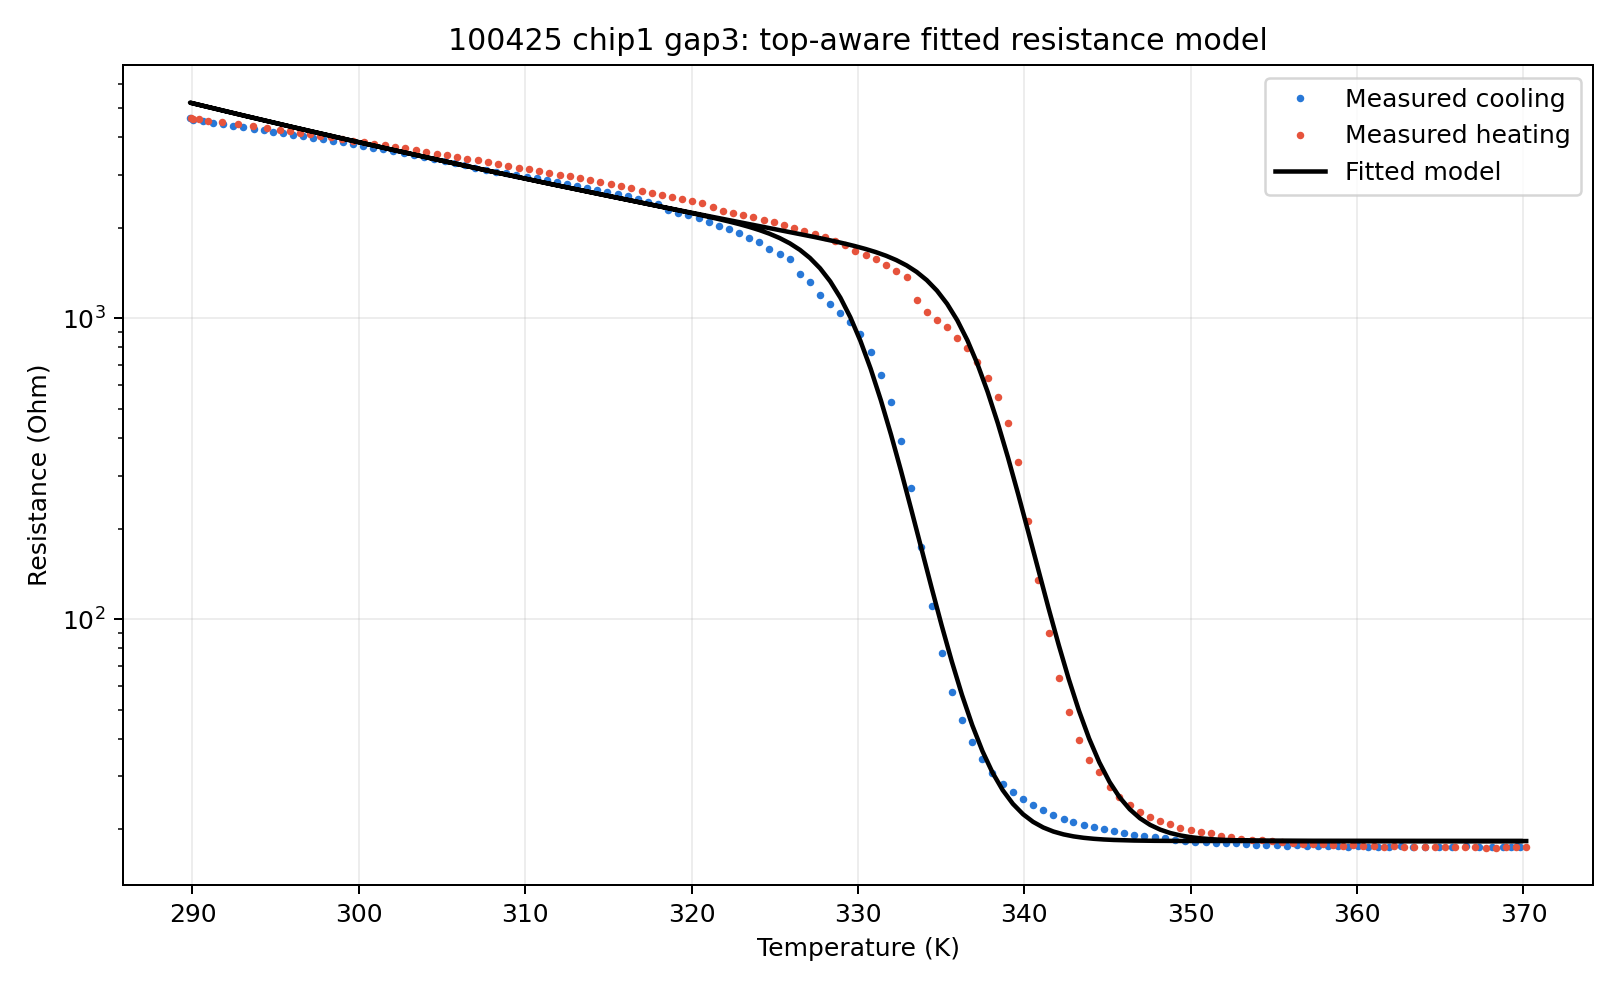
\includegraphics[width=0.78\textwidth]{figures/fit_resistance_rt.png}
\caption{Measured \(R(T)\) points and fitted model for the dataset used in Section 4.}
\label{fig:fit_rt_result}
\end{figure}

\subsubsection*{Limitations}
At the end of this procedure, the following still require additional identification work:
\begin{itemize}
    \item \textbf{Minor-loop fidelity}: one major cooling-heating cycle does not fully constrain history parameters; dedicated reversal experiments are needed.
    \item \textbf{\(\gamma\) identifiability}: with major-loop data only, \(\gamma\) is weakly identifiable, so it is fixed unless additional data is provided.
    \item \textbf{Parameter uniqueness}: different parameter tuples can produce very similar \(\log R(T)\) errors; confidence intervals are not yet computed.
    \item \textbf{Not part of this fit}: electrical/thermal dynamical parameters (\(C\), \(C_{th}\), \(S_e\), source terms) must be calibrated separately from transient simulations.
\end{itemize}

\section{Quasistatic and Dynamic-Phase Current-Source Models}

\subsection{Shared electrothermal equations}
The ideal current-source circuit uses
\begin{align}
C\frac{dV}{dt} &= I_{\mathrm{in}}-\frac{V}{R}, \label{eq:dynamic_current}\\
C_{\mathrm{th}}\frac{dT}{dt} &= \frac{V^2}{R}-S_e(T-T_0). \label{eq:dynamic_thermal}
\end{align}
Both the quasistatic and dynamic-phase models use these same electrical and thermal balances and the same fitted resistance law
\begin{equation}
R(T,g)=R_m+R_0\exp\left(\frac{E_a/k_B}{T}\right)g.
\label{eq:dynamic_resistance}
\end{equation}
The only distinction is how the actual insulating phase fraction \(g\) responds to the hysteresis-prescribed equilibrium fraction \(g_{\mathrm{eq}}(T,\mathcal{H})\).

\subsection{Original quasistatic phase response}
The original Yuanhang Zhang model assumes that the phase fraction responds immediately:
\begin{equation}
g(t)=g_{\mathrm{eq}}\!\left(T(t),\mathcal{H}(t)\right).
\label{eq:official_quasistatic}
\end{equation}
The independent dynamical states are therefore \(V\) and \(T\). Whether a numerical trajectory follows the intended minor-loop geometry also depends on faithful implementation of the discrete reversal detector, as documented below.

A matched quasistatic numerical control also demonstrated why visual inspection of one trace is insufficient. At a reference timestep, several currents showed repeated switching that looked oscillatory. However, changing only the integration timestep caused those cycles to appear, disappear, or change sharply in frequency and amplitude. For example, the \(1100~\mu\mathrm{A}\) control showed repeated cycles at \(dt=0.025~\mathrm{ns}\), no cycles at \(dt=0.05~\mathrm{ns}\), and a different large switching event at finer timesteps. These are apparent numerical oscillations, not a timestep-converged physical limit cycle.

The application History entry \texttt{Quasistatic apparent oscillations - numerical control} preserves these traces with the standard current slider. They were produced by the historical local port bug, not by the exact upstream reversal algorithm.

\subsection{Dynamic-phase working extension}
The local dynamic-phase extension treats \(g\) as a third dynamical state:
\begin{equation}
\tau_g\frac{dg}{dt}=g_{\mathrm{eq}}(T,\mathcal{H})-g.
\label{eq:official_dynamic_phase}
\end{equation}
The resistance in Equation~\ref{eq:dynamic_resistance} is evaluated using this delayed \(g(t)\). The quasistatic model is recovered as \(\tau_g\rightarrow 0\).

Practically, finite \(\tau_g\) means that temperature first changes the preferred phase fraction, while the actual material state and resistance respond later. This introduces a delayed feedback loop:
\[
I_{\mathrm{in}}\rightarrow V\rightarrow P_{\mathrm{Joule}}\rightarrow T
\rightarrow g_{\mathrm{eq}}\rightarrow g\rightarrow R\rightarrow V.
\]
The delay can support a limit cycle even when the corresponding instantaneous-feedback model approaches a fixed point. This extension is physically motivated by finite transition kinetics, but it is not part of the original Yuanhang Zhang repository and must be independently calibrated before its quantitative predictions are treated as experimental predictions.

\begin{table}[htbp]
\centering
\small
\caption{Direct comparison of the two phase-response assumptions.}
\label{tab:phase_model_comparison}
\begin{tabular}{p{0.25\textwidth}p{0.31\textwidth}p{0.31\textwidth}}
\toprule
Property & Quasistatic model & Dynamic-phase extension \\
\midrule
Independent states & \(V,T\) & \(V,T,g\) \\
Phase response & \(g=g_{\mathrm{eq}}(T,\mathcal{H})\) & \(\tau_g\dot g=g_{\mathrm{eq}}-g\) \\
New parameter & none & \(\tau_g\) \\
Original Yuanhang code & yes & no \\
Current-source result after reversal-detector fix & a newly targeted parameter set supports a converged relaxation-oscillation domain & tested prior candidate points approach fixed points \\
\bottomrule
\end{tabular}
\end{table}

\section{Dynamic-Model Article-Comparison Campaign}

\subsection{Target observables}
The comparison preprint supplied for this project reports a current-driven oscillatory regime at approximately \(200\)--\(600~\mu\mathrm{A}\), oscillation frequencies near \(40\)--\(60~\mathrm{MHz}\), mean power near \(60\)--\(100~\mu\mathrm{W}\), and energy near \(1.2\)--\(1.9~\mathrm{pJ}\) per cycle. These values were used as targets, not as fitted constraints.

\subsection{Search procedure}
The search kept the resistance model and dynamic-phase equations unchanged. It:
\begin{enumerate}
    \item used the improved measured-sample resistance fits;
    \item broadly sampled \(C\), \(C_{\mathrm{th}}\), \(S_e\), \(\tau_g\), and \(T_0\);
    \item first screened the center of the reported current window;
    \item tested neighboring currents only after a candidate showed repeated cycles; and
    \item required late-window persistence and repeated simulations at smaller timesteps before accepting a result.
\end{enumerate}

Across the four newly fitted samples and the best-characterized 100425 chip1 gap3 sample, the broad \(200\)--\(600~\mu\mathrm{A}\) searches produced large switching transients but no sustained \(40\)--\(60~\mathrm{MHz}\) limit cycle.

At a higher-current exploratory base point,
\[
C=80~\mathrm{pF},\quad
C_{\mathrm{th}}=3~\mathrm{pJ/K},\quad
S_e=0.052838~\mathrm{mW/K},\quad
\tau_g=10~\mathrm{ns},\quad
T_0=325~\mathrm{K},
\]
coarser integrations using the historical local per-step port showed apparent late-time oscillations over parts of approximately \(0.8\)--\(1.8~\mathrm{mA}\), with frequencies of roughly \(4.7\)--\(10.1~\mathrm{MHz}\). These legacy results did not quantitatively reproduce the preprint's current or frequency range and did not survive corrected reversal handling.

\begin{figure}[H]
\centering
\includegraphics[width=0.96\textwidth]{../../outputs/dynamic_article_comparison/sweep_frequency_summary.png}
\caption{Legacy one-at-a-time dynamic-phase sweeps generated with the timestep-dependent local port bug. Green points passed the late-window criterion at the screening timestep, but the apparent oscillations did not survive corrected reversal handling.}
\label{fig:dynamic_article_sweeps}
\end{figure}

\subsection{Timestep-convergence audit and numerical correction}
The apparent oscillatory domains were tested over \(5~\mu\mathrm{s}\) at timesteps of \(0.05\), \(0.025\), and \(0.0125~\mathrm{ns}\). The \(0.05\) and \(0.025~\mathrm{ns}\) results were often close, but the \(0.0125~\mathrm{ns}\) results changed sharply in frequency and voltage amplitude. Therefore, the apparent domains are not yet timestep-converged.

The sensitivity was associated with a bug in the local port of the hysteresis reversal detector. The port updated its temperature anchor after every numerical step, so a reversal was accepted only when the temperature change in one integration step exceeded the fixed threshold
\begin{equation}
|\Delta T_{\mathrm{step}}|>0.01~\mathrm{K}.
\label{eq:reversal_step_threshold}
\end{equation}
Changing the timestep changes \(\Delta T_{\mathrm{step}}\), and therefore changed whether and when the hysteresis branch reversed. This was not faithful to Yuanhang Zhang's source code. Upstream updates its anchor only after accumulated displacement exceeds \(0.01~\mathrm{K}\).

Two corrected modes are now explicit. The default \texttt{yuanhang\_reference} mode faithfully implements upstream accumulated-displacement and sampled detection-point geometry. The optional \texttt{turning\_point} extension tracks the latest temperature extremum \(T_{\mathrm{extreme}}\) and confirms a reversal after the cumulative excursion satisfies
\begin{equation}
\left|T-T_{\mathrm{extreme}}\right|>0.01~\mathrm{K}.
\label{eq:reversal_cumulative_threshold}
\end{equation}
In the extension, the reversal point is assigned to \(T_{\mathrm{extreme}}\), rather than to the sampled detection point used upstream. This makes the extension timestep robust but changes minor-loop geometry. A third mode, \texttt{ported\_per\_step}, is retained only to reproduce historical artifacts and must not be used for new physical claims.

\begin{figure}[H]
\centering
\includegraphics[width=0.92\textwidth]{../../jobs/20260614_125407_article_audit_816bf1/timestep_convergence_audit.png}
\caption{Legacy timestep-convergence audit for representative apparent oscillatory points. The frequency and amplitude changes exposed the local anchor-update bug and motivated a full upstream-fidelity audit.}
\label{fig:dynamic_convergence_audit}
\end{figure}

\subsection{Post-correction convergence results}
The measured 100425 resistance-fit RMSE remained effectively unchanged at \(0.03733344\), showing that the numerical correction did not disturb the fitted major resistance loop.

After the correction, the previously tested quasistatic and dynamic-phase current-source candidate points at \(800\), \(1100\), \(1500\), and \(1800~\mu\mathrm{A}\) all approached fixed points consistently for \(dt=0.05\), \(0.025\), \(0.0125\), and \(0.00625~\mathrm{ns}\). The previously reported domains at those parameter sets must therefore be classified as numerical artifacts of the legacy reversal detector.

A subsequent first-principles search using the \texttt{turning\_point} reversal extension found a different, timestep-converged oscillatory domain while retaining the original quasistatic ideal-current equations and fixed measured resistance fit. The search targeted the steep negative-slope portion of the fitted heating branch. At a current-source equilibrium,
\begin{equation}
I^2R(T)=S_e(T-T_0),
\end{equation}
and the local \(V,T\) Jacobian can become an unstable focus when the negative \(dR/dT\) feedback overcomes electrical and thermal damping. Simulating parameter sets selected from this condition identified
\[
C=25.930953~\mathrm{pF},\quad
C_{\mathrm{th}}=5.0~\mathrm{pJ/K},\quad
S_e=0.1~\mathrm{mW/K},\quad
T_0=311.219374~\mathrm{K}.
\]
For the measured 100425 chip1 gap3 resistance fit, that extension produced sustained quasistatic relaxation oscillations from approximately \(1.27\) to \(2.74~\mathrm{mA}\). Fixed points were recovered at \(1.20\) and \(2.80~\mathrm{mA}\). Across the extension's oscillatory domain, frequency increased from approximately \(5.49\) to \(14.13~\mathrm{MHz}\). A subsequent exact-reference resweep found a narrower upper edge: sustained late-window oscillations remained at \(2.47~\mathrm{mA}\), while \(2.48~\mathrm{mA}\) settled to a fixed point.

At \(I=1640.226~\mu\mathrm{A}\), the period converges as the timestep is halved:
\begin{center}
\begin{tabular}{rrr}
\toprule
\(dt\) (ns) & Period (ns) & Frequency (MHz) \\
\midrule
0.015820 & 123.206 & 8.116 \\
0.007910 & 123.135 & 8.121 \\
0.003955 & 123.095 & 8.124 \\
\bottomrule
\end{tabular}
\end{center}
The late-window voltage peak-to-peak amplitude converges near \(2.275~\mathrm{V}\), and the temperature remains approximately \(325.4\)--\(349.1~\mathrm{K}\). The application History entry \texttt{Validated old-model quasistatic oscillatory domain} preserves fixed-point controls and representative traces, but its name predates the fidelity audit: those saved traces used the \texttt{turning\_point} extension.

As a positive control, the original voltage-driven relaxation oscillator remained oscillatory and converged as the timestep was reduced:
\begin{center}
\begin{tabular}{rrr}
\toprule
\(dt\) (ns) & Frequency (MHz) & Voltage peak-to-peak (V) \\
\midrule
10.00 & 0.4330 & 5.012 \\
5.00 & 0.4372 & 4.921 \\
2.50 & 0.4395 & 4.873 \\
1.25 & 0.4407 & 4.849 \\
\bottomrule
\end{tabular}
\end{center}
This is the expected signature of a robust circuit-driven oscillation: the behavior persists and its quantitative values approach stable limits as \(dt\) decreases.

\subsection{Current scientific conclusion}
The quasistatic ideal-current equations support a broad, timestep-converged relaxation-oscillation domain when the electrical and thermal timescales are selected from the instability condition on the measured resistance transition. The sole supported hysteresis implementation is now the exact Yuanhang reference detector, for which the audited sweep extends through approximately \(2.47~\mathrm{mA}\) and reaches a fixed point at \(2.48~\mathrm{mA}\). The former turning-point extension produced an historical upper boundary near \(2.74~\mathrm{mA}\), but it was removed from executable code because it changed minor-loop geometry. The dynamic-phase extension remains a physically plausible hypothesis, but the searched dynamic-phase parameter sets have not yet produced a separately validated current-source limit cycle. Specifically:
\begin{itemize}
    \item the searched model did not reproduce the supplied preprint's \(200\)--\(600~\mu\mathrm{A}\), \(40\)--\(60~\mathrm{MHz}\) domain;
    \item the old candidate domains disappeared after correcting timestep-dependent reversal recognition;
    \item an historical turning-point search found a different domain, but that reversal extension is no longer executable;
    \item the exact-reference resweep found oscillations through \(2.47~\mathrm{mA}\) and a fixed point at \(2.48~\mathrm{mA}\);
    \item the exact upstream float32 hysteresis path is now the only software implementation and matches the vendored reference trace to within \(0.001~\Omega\) on the fidelity audit;
    \item the original voltage-driven oscillator survives and converges under the same correction; and
    \item all future positive domains must continue to pass corrected-detector timestep and duration checks.
\end{itemize}

Legacy exploratory traces remain saved in the application History and are explicitly labeled as pre-correction numerical results. Their obsolete mode fields are provenance only; rerunning a historical configuration uses the sole Yuanhang reference implementation.

\section{Sources}
\begin{enumerate}
    \item Y.-H. Zhang \emph{et al.}, ``Collective dynamics and long-range order in thermal neuristor networks,'' \emph{Nature Communications}, 2024.
    \item L. A. L. de Almeida \emph{et al.}, ``Modeling of the hysteretic metal-insulator transition in a vanadium dioxide infrared detector,'' \emph{Optical Engineering}, 2002.
    \item R. Hooke and T. A. Jeeves, ``Direct Search'' Solution of Numerical and Statistical Problems,'' \emph{Journal of the ACM}, vol. 8, no. 2, pp. 212--229, 1961.
    \item T. G. Kolda, R. M. Lewis, and V. Torczon, ``Optimization by Direct Search: New Perspectives on Some Classical and Modern Methods,'' \emph{SIAM Review}, vol. 45, no. 3, pp. 385--482, 2003.
    \item A. R. Conn, K. Scheinberg, and L. N. Vicente, \emph{Introduction to Derivative-Free Optimization}. SIAM, 2009.
    \item ``Harnessing the VO2 Phase Transition for Automatic Gain Control in Transimpedance Amplifiers,'' preprint arXiv:2604.04594, 2026.
\end{enumerate}

\end{document}
